\begin{figure}[H]
    \centering
    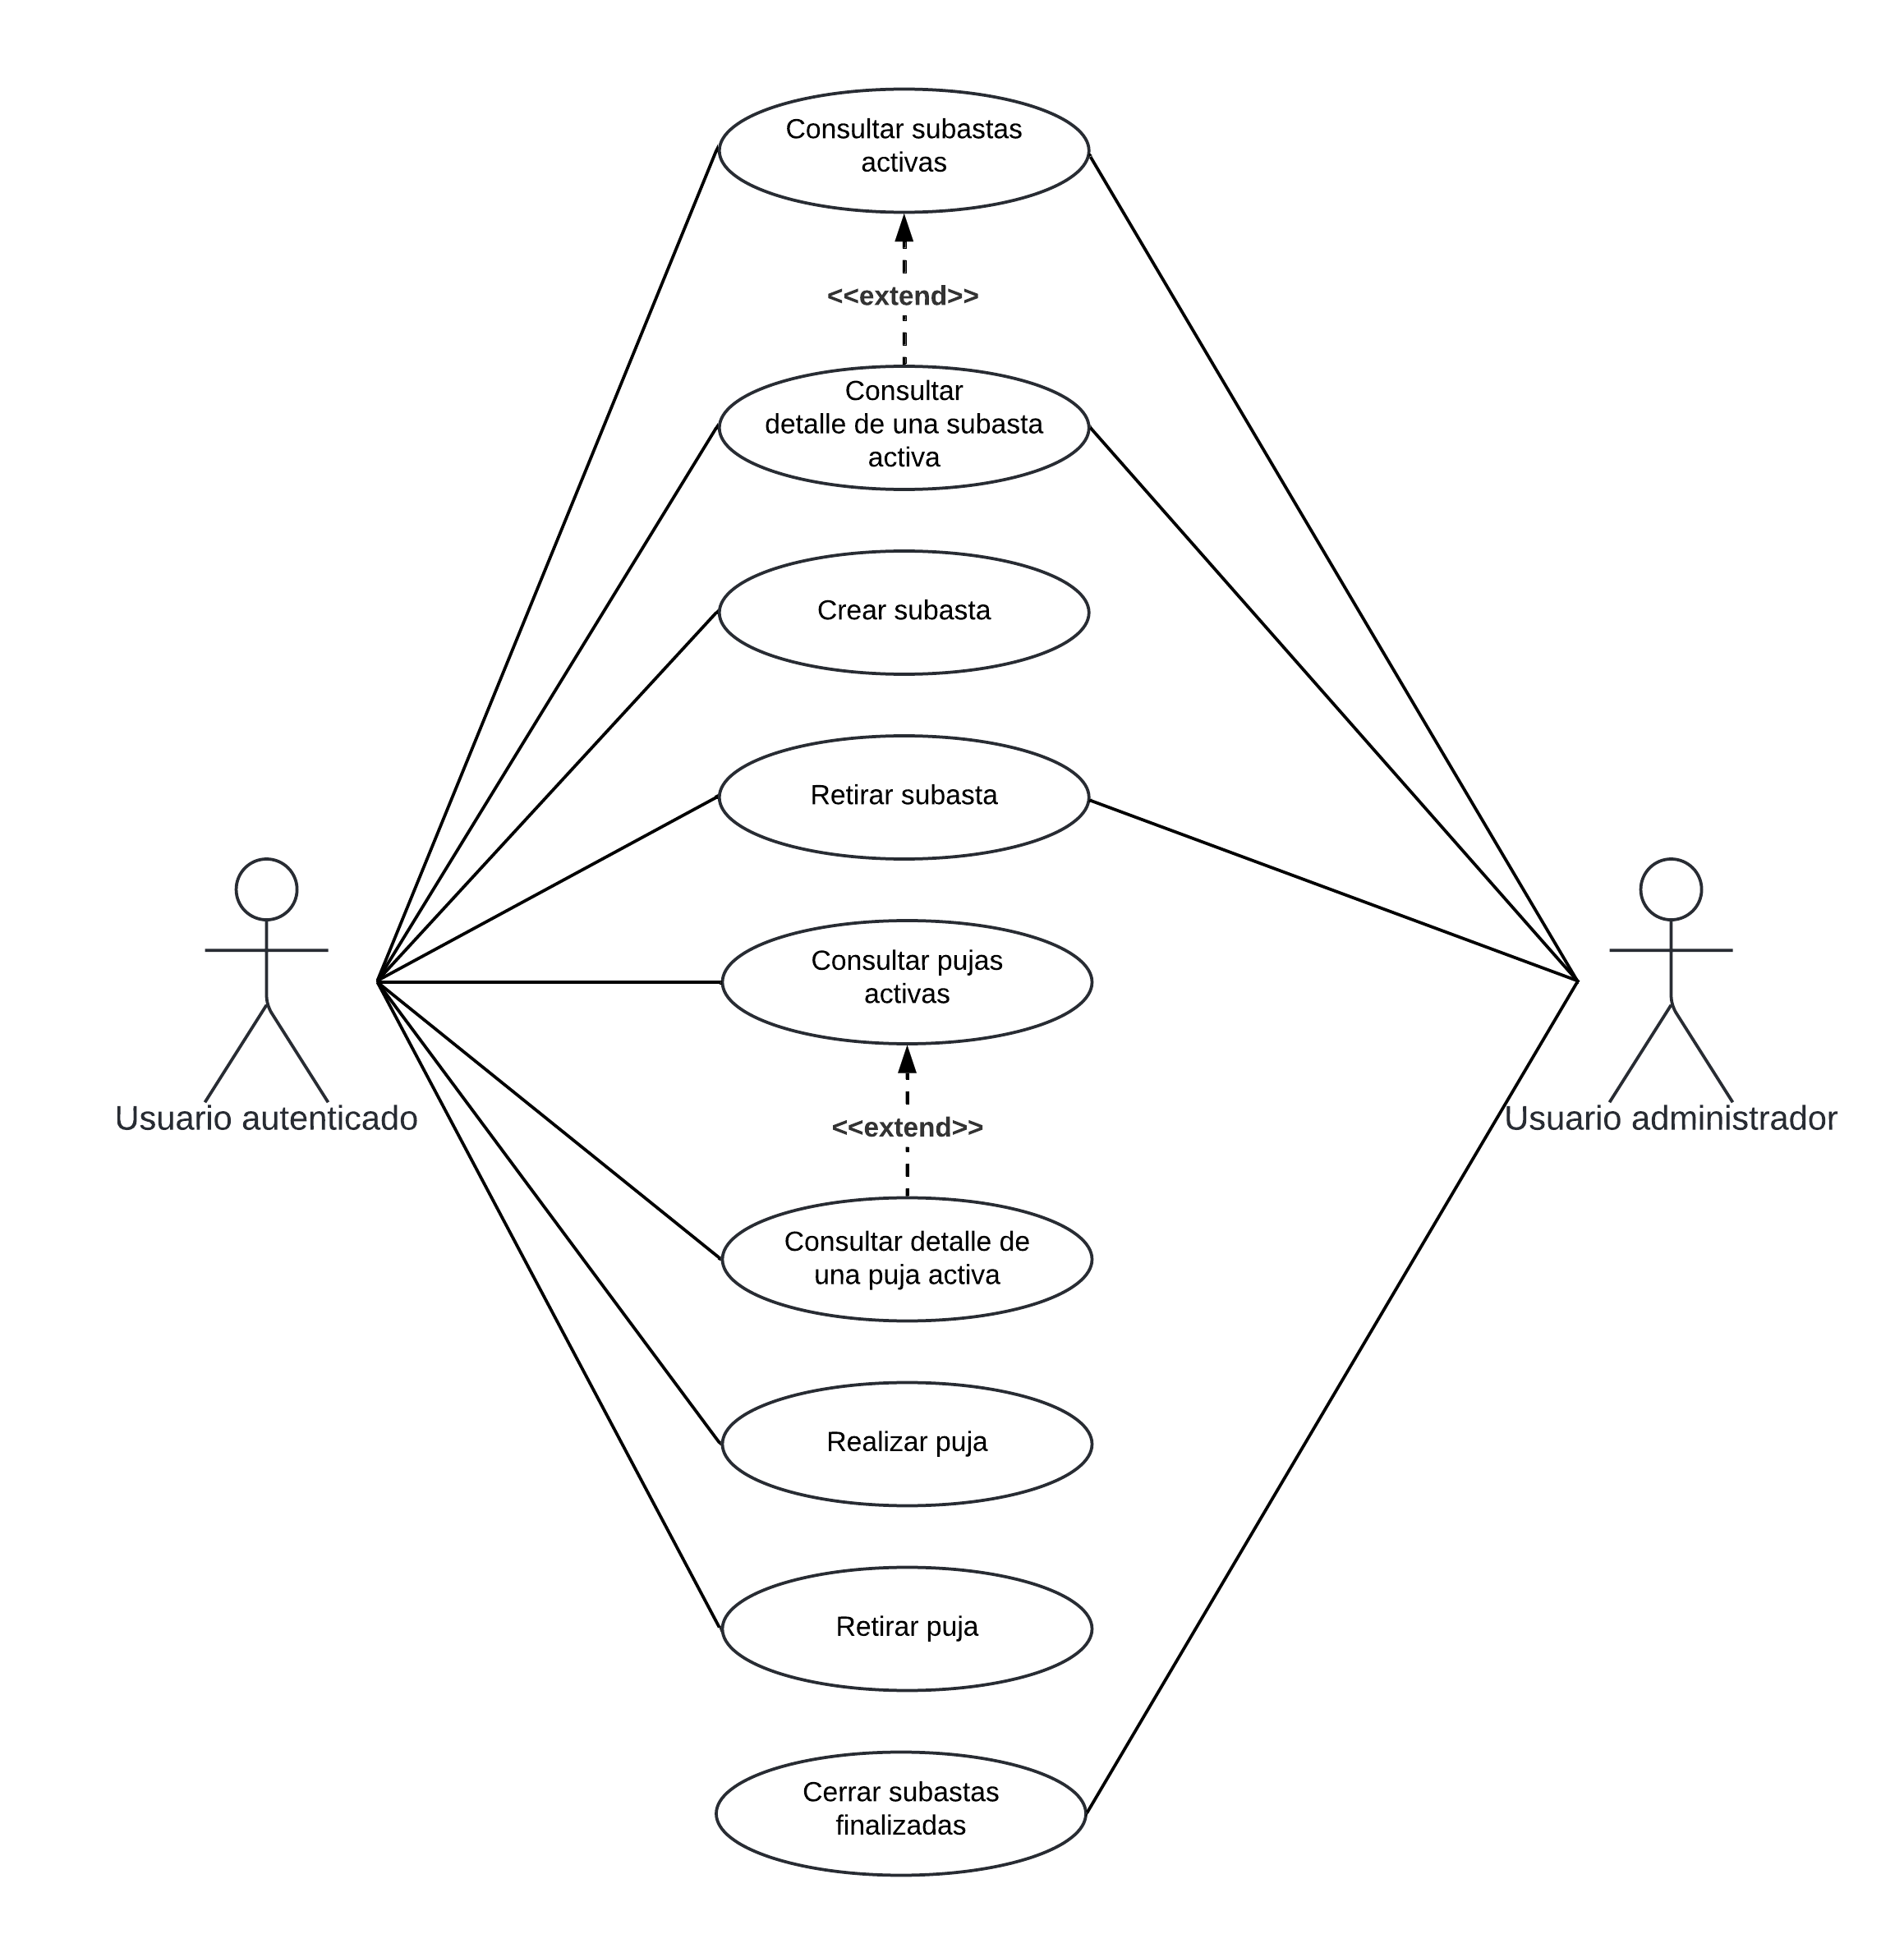
\includegraphics[width=0.5\textwidth]{figures/6-Analisis/6-Casos-uso/6_3_4_Gestion-subastas-pujas.png}
    \caption{Casos de uso. Gestión de subastas y pujas}
    \label{fig:cu_gestion-subastas-pujas}
\end{figure}

\subsubsection{Caso de uso. Crear una subasta} \label{sec:cu_crear-subasta}
\begin{longtable}{
    >{\columncolor{lightgreen!20}}p{4cm}
    p{12cm}
    }
    \caption{Caso de uso. Crear una subasta} \label{table:cu_crear-subasta} \\
    \toprule
    \rowcolor{darkgreen!50}
    \textbf{Caso de uso} & \multicolumn{1}{>{\columncolor{darkgreen!50}\centering\arraybackslash}p{12cm}}{\textbf{CREAR UNA SUBASTA}} \\
    \endfirsthead
    
    \multicolumn{2}{c}%
    {{ \tablename\ \thetable{} Caso de uso. Crear una subasta -- continuación de la página anterior}} \\
    \toprule
    \rowcolor{darkgreen!50}
    \textbf{Caso de uso} & \multicolumn{1}{>{\columncolor{darkgreen!50}\centering\arraybackslash}p{12cm}}{\textbf{CREAR UNA SUBASTA}} \\
    \midrule
    \endhead
    
    \midrule
    \multicolumn{2}{r}{{Continúa en la siguiente página...}} \\ 
    \endfoot
    
    \bottomrule
    \endlastfoot
    
    \midrule
    Descripción & Un usuario autenticado puede crear una subasta de una carta de su colección. \\
    \midrule
    Actores principales & Usuario autenticado \\
    \midrule
    Actores secundarios &  \\
    \midrule
    Precondiciones & \begin{itemize}[nosep,leftmargin=*]
        \item El usuario debe haber iniciado sesión en el sistema.
        \item El usuario debe tener al menos una carta en su colección.
        \item El usuario no debe tener ya una subasta activa para la carta que desea subastar.
    \end{itemize} \\
    \midrule
    Postcondiciones & \begin{itemize}[nosep,leftmargin=*]
        \item Se crea una nueva subasta en la base de datos.
        \item Se marca la carta como 'en subasta' en la base de datos.
    \end{itemize} \\
    \midrule
    Disparadores & El usuario accede a la sección de subastas y hace clic en el botón de crear subasta. \\
    \midrule
    Escenario principal & \begin{enumerate}[nosep,leftmargin=*]
        \item El sistema muestra el formulario de creación de subasta.
        \item El usuario selecciona la carta que desea subastar.
        \item El usuario introduce el precio de salida y la duración de la subasta.
        \item El usuario hace clic en el botón de crear subasta.
        \item El sistema valida los campos del formulario.
        \item El sistema crea una nueva subasta en la base de datos.
        \item El sistema marca la carta como 'en subasta' en la base de datos.
        \item El sistema muestra un mensaje de éxito.
        \item El sistema redirige al usuario a la página de subastas.
        \item El sistema muestra la subasta creada en la lista de subastas.
    \end{enumerate} \\
    \midrule
    Escenarios alternativos & 
    \begin{itemize}[nosep,leftmargin=*]
        \item \textbf{Escenario alternativo 1. El usuario ya tiene una subasta activa para la carta que desea subastar.}
        \begin{enumerate}[nosep,leftmargin=*]
            \item El usuario intenta crear una subasta para una carta que ya está en subasta.
            \item El sistema muestra un mensaje de error.
            \item El sistema redirige al usuario a la página de subastas.
        \end{enumerate}
        \item \textbf{Escenario alternativo 2. El usuario introduce datos inválidos.}
        \begin{enumerate}[nosep,leftmargin=*]
            \item El sistema muestra un mensaje de error.
            \item El sistema no crea la subasta en la base de datos.
            \item El sistema no marcará la carta como 'en subasta' en la base de datos.
            \item El sistema le mostrará al usuario los campos con errores.
            \item El sistema permitirá al usuario corregir los errores.
        \end{enumerate}
    \end{itemize} \\
    \midrule
    Situaciones de error & 
    \begin{itemize}[nosep,leftmargin=*]
        \item \textbf{Error de conexión a la base de datos.}
        \begin{enumerate}[nosep,leftmargin=*]
            \item El sistema mostrará un mensaje de error.
            \item El sistema no creará la subasta en la base de datos.
            \item El sistema no marcará la carta como 'en subasta' en la base de datos.
            \item El sistema redirigirá al usuario a la página de subastas.
        \end{enumerate}
    \end{itemize} \\
\end{longtable}




\subsubsection{Caso de uso. Retirar una subasta} \label{sec:cu_retirar-subasta}
\begin{longtable}{
    >{\columncolor{lightgreen!20}}p{4cm}
    p{12cm}
    }
    \caption{Caso de uso. Retirar una subasta} \label{table:cu_retirar-subasta} \\
    \toprule
    \rowcolor{darkgreen!50}
    \textbf{Caso de uso} & \multicolumn{1}{>{\columncolor{darkgreen!50}\centering\arraybackslash}p{12cm}}{\textbf{RETIRAR UNA SUBASTA}} \\
    \endfirsthead
    
    \multicolumn{2}{c}%
    {{ \tablename\ \thetable{} Caso de uso. Retirar una subasta -- continuación de la página anterior}} \\
    \toprule
    \rowcolor{darkgreen!50}
    \textbf{Caso de uso} & \multicolumn{1}{>{\columncolor{darkgreen!50}\centering\arraybackslash}p{12cm}}{\textbf{RETIRAR UNA SUBASTA}} \\
    \midrule
    \endhead
    
    \midrule
    \multicolumn{2}{r}{{Continúa en la siguiente página...}} \\ 
    \endfoot
    
    \bottomrule
    \endlastfoot
    
    \midrule
    Descripción & Un usuario autenticado puede retirar una subasta activa en el sistema si es el vendedor de la subasta. Un usuario administrador puede retirar cualquier subasta activa en el sistema. \\
    \midrule
    Actores principales & Usuario autenticado o usuario administrador \\
    \midrule
    Actores secundarios &  \\
    \midrule
    Precondiciones & \begin{itemize}[nosep,leftmargin=*]
        \item El usuario debe haber iniciado sesión en el sistema.
        \item El usuario debe tener al menos una subasta activa.
    \end{itemize} \\
    \midrule
    Postcondiciones & \begin{itemize}[nosep,leftmargin=*]
        \item Se marca la subasta como 'cancelada' en la base de datos.
        \item La carta subastada vuelve a estar disponible en la colección del usuario.
        \item Se actualizan las pujas de la subasta en la base de datos, marcando las pujas como 'canceladas'.
        \item Se informa a los usuarios que hayan pujado en la subasta de que ha sido cancelada.
        \item Si la subasta ha sido retirada por un administrador, se notifica al usuario vendedor de la subasta en tiempo real.
    \end{itemize} \\
    \midrule
    Disparadores & El usuario accede a la sección de subastas y hace clic en el botón de retirar subasta. \\
    \midrule
    Escenario principal & \begin{enumerate}[nosep,leftmargin=*]
        \item El sistema muestra la lista de subastas activas del usuario.
        \item El usuario selecciona la subasta que desea retirar.
        \item El usuario hace clic en el botón de retirar subasta.
        \item El sistema muestra un mensaje de confirmación.
        \item El usuario confirma la retirada de la subasta.
        \item El sistema marca la subasta como 'cancelada' en la base de datos.
        \item La carta subastada vuelve a estar disponible en la colección del usuario.
        \item El sistema muestra un mensaje de éxito.
        \item El sistema redirige al usuario a la página de subastas.
    \end{enumerate} \\
    \midrule
    Escenarios alternativos & 
    \begin{itemize}[nosep,leftmargin=*]
        \item \textbf{Escenario alternativo 1. El usuario cancela la retirada de la subasta.}
        \begin{enumerate}[nosep,leftmargin=*]
            \item El usuario hace clic en el botón de cancelar en el mensaje de confirmación.
            \item El sistema no marcará la subasta como 'cancelada' en la base de datos.
            \item El sistema redirigirá al usuario a la página de subastas.
        \end{enumerate}
    \end{itemize} \\
    \midrule
    Situaciones de error & 
    \begin{itemize}[nosep,leftmargin=*]
        \item \textbf{Error de conexión a la base de datos.}
        \begin{enumerate}[nosep,leftmargin=*]
            \item El sistema mostrará un mensaje de error.
            \item El sistema no marcará la subasta como 'cancelada' en la base de datos.
            \item El sistema no devolverá la carta subastada a la colección del usuario.
            \item El sistema redirigirá al usuario a la página de subastas.
        \end{enumerate}
    \end{itemize} \\
\end{longtable}




\subsubsection{Caso de uso. Consultar subastas activas} \label{sec:cu_consultar-subastas}
\begin{longtable}{
    >{\columncolor{lightgreen!20}}p{4cm}
    p{12cm}
    }
    \caption{Caso de uso. Consultar subastas activas} \label{table:cu_consultar-subastas} \\
    \toprule
    \rowcolor{darkgreen!50}
    \textbf{Caso de uso} & \multicolumn{1}{>{\columncolor{darkgreen!50}\centering\arraybackslash}p{12cm}}{\textbf{CONSULTAR SUBASTAS ACTIVAS}} \\
    \endfirsthead
    
    \multicolumn{2}{c}%
    {{ \tablename\ \thetable{} Caso de uso. Consultar subastas activas -- continuación de la página anterior}} \\
    \toprule
    \rowcolor{darkgreen!50}
    \textbf{Caso de uso} & \multicolumn{1}{>{\columncolor{darkgreen!50}\centering\arraybackslash}p{12cm}}{\textbf{CONSULTAR SUBASTAS ACTIVAS}} \\
    \midrule
    \endhead
    
    \midrule
    \multicolumn{2}{r}{{Continúa en la siguiente página...}} \\ 
    \endfoot
    
    \bottomrule
    \endlastfoot
    
    \midrule
    Descripción & Un usuario autenticado o administrador puede consultar las subastas activas en el sistema. \\
    \midrule
    Actores principales & Usuario autenticado o usuario administrador \\
    \midrule
    Actores secundarios &  \\
    \midrule
    Precondiciones & \begin{itemize}[nosep,leftmargin=*]
        \item El usuario debe haber iniciado sesión en el sistema.
    \end{itemize} \\
    \midrule
    Postcondiciones &  \\
    \midrule
    Disparadores & El usuario accede a la sección de subastas. \\
    \midrule
    Escenario principal & \begin{enumerate}[nosep,leftmargin=*]
        \item El sistema muestra la lista de subastas activas.
        \item El usuario puede seleccionar una subasta para ver su información detallada.
    \end{enumerate} \\
    \midrule
    Escenarios alternativos & 
    \begin{itemize}[nosep,leftmargin=*]
        \item \textbf{Escenario alternativo 1. No hay subastas activas.}
        \begin{enumerate}[nosep,leftmargin=*]
            \item El sistema mostrará un mensaje indicando que no hay subastas activas.
        \end{enumerate}
        \item \textbf{Escenario alternativo 2. El usuario consulta sus propias subastas.} 
        \begin{enumerate}[nosep,leftmargin=*]
            \item El usuario accede a la sección de subastas.
            \item El sistema muestra la opción de ver las subastas activas del usuario.
            \item El usuario selecciona la opción de ver sus propias subastas.
            \item El sistema muestra la lista de subastas activas del usuario.
            \item El usuario puede seleccionar una subasta para ver su información detallada.
        \end{enumerate}
        \item \textbf{Escenario alternativo 3. Un usuario administrador consulta las subastas activas.}
        \begin{enumerate}[nosep,leftmargin=*]
            \item El usuario administrador accede a la sección de subastas.
            \item El sistema muestra la lista de subastas activas de todos los usuarios.
            \item El usuario administrador puede seleccionar una subasta para ver su información detallada.
        \end{enumerate}
    \end{itemize} \\
    \midrule
    Situaciones de error & 
    \begin{itemize}[nosep,leftmargin=*]
        \item \textbf{Error de conexión a la base de datos.}
        \begin{enumerate}[nosep,leftmargin=*]
            \item El sistema mostrará un mensaje de error.
        \end{enumerate}
    \end{itemize} \\
\end{longtable}

\subsubsection{Caso de uso. Consultar el detalle de una subasta activa} \label{sec:cu_consultar-detalle-subasta}
\begin{longtable}{
    >{\columncolor{lightgreen!20}}p{4cm}
    p{12cm}
    }
    \caption{Caso de uso. Consultar el detalle de una subasta activa} \label{table:cu_consultar-detalle-subasta} \\
    \toprule
    \rowcolor{darkgreen!50}
    \textbf{Caso de uso} & \multicolumn{1}{>{\columncolor{darkgreen!50}\centering\arraybackslash}p{12cm}}{\textbf{CONSULTAR DETALLE DE UNA SUBASTA ACTIVA}} \\
    \endfirsthead
    
    \multicolumn{2}{c}%
    {{ \tablename\ \thetable{} Caso de uso. Consultar el detalle de una subasta activa -- continuación de la página anterior}} \\
    \toprule
    \rowcolor{darkgreen!50}
    \textbf{Caso de uso} & \multicolumn{1}{>{\columncolor{darkgreen!50}\centering\arraybackslash}p{12cm}}{\textbf{CONSULTAR DETALLE DE UNA SUBASTA ACTIVA}} \\
    \midrule
    \endhead
    
    \midrule
    \multicolumn{2}{r}{{Continúa en la siguiente página...}} \\ 
    \endfoot
    
    \bottomrule
    \endlastfoot
    
    \midrule
    Descripción & Un usuario autenticado o administrador puede consultar el detalle de una subasta activa en el sistema. \\
    \midrule
    Actores principales & Usuario autenticado o usuario administrador \\
    \midrule
    Actores secundarios &  \\
    \midrule
    Precondiciones & \begin{itemize}[nosep,leftmargin=*]
        \item El usuario debe haber iniciado sesión en el sistema.
    \end{itemize} \\
    \midrule
    Postcondiciones &  \\
    \midrule
    Disparadores & El usuario accede a la sección de subastas y selecciona una subasta activa. \\
    \midrule
    Escenario principal & \begin{enumerate}[nosep,leftmargin=*]
        \item El usuario selecciona una subasta activa.
        \item El sistema muestra la información detallada de la carta subastada, incluido el histórico de transacciones de esta.
        \item El sistema muestra la duración restante de la subasta.
    \end{enumerate} \\
    \midrule
    Escenarios alternativos & 
    \begin{itemize}[nosep,leftmargin=*]
        \item \textbf{Escenario alternativo 1. El usuario que consulta la subasta es el propietario de la subasta.}
        \begin{enumerate}[nosep,leftmargin=*]
            \item El usuario selecciona una subasta activa.
            \item El sistema muestra la información detallada de la carta subastada, incluido el histórico de transacciones de esta.
            \item El sistema muestra la duración restante de la subasta.
            \item El sistema muestra el precio de salida establecido por el usuario.
            \item El sistema muestra la opción de retirar la subasta.
        \end{enumerate}
        \item \textbf{Escenario alternativo 3. Un usuario administrador consulta la subasta.}
        \begin{enumerate}[nosep,leftmargin=*]
            \item El usuario administrador selecciona una subasta activa.
            \item El sistema muestra la información detallada de la carta subastada, incluido el histórico de transacciones de esta.
            \item El sistema muestra la duración restante de la subasta.
            \item El sistema muestra el precio de salida establecido por el vendedor.
            \item El sistema muestra la opción de retirar la subasta.
        \end{enumerate}
    \end{itemize} \\
    \midrule
    Situaciones de error & 
    \begin{itemize}[nosep,leftmargin=*]
        \item \textbf{Error de conexión a la base de datos.}
        \begin{enumerate}[nosep,leftmargin=*]
            \item El sistema mostrará un mensaje de error.
        \end{enumerate}
    \end{itemize} \\
\end{longtable}


\subsubsection{Caso de uso. Realizar puja} \label{sec:cu_realizar-puja}
\begin{longtable}{
    >{\columncolor{lightgreen!20}}p{4cm}
    p{12cm}
    }
    \caption{Caso de uso. Realizar puja} \label{table:cu_realizar-puja} \\
    \toprule
    \rowcolor{darkgreen!50}
    \textbf{Caso de uso} & \multicolumn{1}{>{\columncolor{darkgreen!50}\centering\arraybackslash}p{12cm}}{\textbf{REALIZAR PUJA}} \\
    \endfirsthead
    
    \multicolumn{2}{c}%
    {{ \tablename\ \thetable{} Caso de uso. Realizar puja -- continuación de la página anterior}} \\
    \toprule
    \rowcolor{darkgreen!50}
    \textbf{Caso de uso} & \multicolumn{1}{>{\columncolor{darkgreen!50}\centering\arraybackslash}p{12cm}}{\textbf{REALIZAR PUJA}} \\
    \midrule
    \endhead
    
    \midrule
    \multicolumn{2}{r}{{Continúa en la siguiente página...}} \\ 
    \endfoot
    
    \bottomrule
    \endlastfoot
    
    \midrule
    Descripción & Un usuario autenticado puede realizar una puja en una subasta activa. \\
    \midrule
    Actores principales & Usuario autenticado \\
    \midrule
    Actores secundarios &  \\
    \midrule
    Precondiciones & \begin{itemize}[nosep,leftmargin=*]
        \item El usuario debe haber iniciado sesión en el sistema.
        \item El usuario debe tener saldo suficiente para realizar la puja.
    \end{itemize} \\
    \midrule
    Postcondiciones & \begin{itemize}[nosep,leftmargin=*]
        \item Se registra la puja en la base de datos.
    \end{itemize} \\
    \midrule
    Disparadores & El usuario selecciona una subasta activa y hace clic en el botón de realizar puja. \\
    \midrule
    Escenario principal & \begin{enumerate}[nosep,leftmargin=*]
        \item El sistema muestra la información detallada de la subasta.
        \item El usuario introduce la cantidad de la puja.
        \item El usuario hace clic en el botón de realizar puja.
        \item El sistema valida la cantidad de la puja.
        \item El sistema registra la puja en la base de datos.
        \item El sistema muestra un mensaje de éxito.
        \item El sistema muestra un mensaje informativo, indicando que si en el momento de finalización del tiempo de la subasta no cuenta con el saldo suficiente, la puja no será válida.
        \item El sistema redirige al usuario a la página de subastas.
    \end{enumerate} \\
    \midrule
    Escenarios alternativos & 
    \begin{itemize}[nosep,leftmargin=*]
        \item \textbf{Escenario alternativo 1. El usuario no tiene saldo suficiente para realizar la puja.}
        \begin{enumerate}[nosep,leftmargin=*]
            \item El usuario intenta realizar una puja sin tener saldo suficiente.
            \item El sistema mostrará un mensaje de error.
            \item El sistema no registrará la puja en la base de datos.
            \item El sistema redirigirá al usuario a la página de subastas.
        \end{enumerate}
        \item \textbf{Escenario alternativo 2. El usuario introduce una cantidad de puja inválida.}
        \begin{enumerate}[nosep,leftmargin=*]
            \item El sistema mostrará un mensaje de error.
            \item El sistema no registrará la puja en la base de datos.
            \item El sistema le mostrará al usuario los campos con errores.
            \item El sistema permitirá al usuario corregir los errores.
        \end{enumerate}
    \end{itemize} \\
    \midrule
    Situaciones de error & 
    \begin{itemize}[nosep,leftmargin=*]
        \item \textbf{Error de conexión a la base de datos.}
        \begin{enumerate}[nosep,leftmargin=*]
            \item El sistema mostrará un mensaje de error.
            \item El sistema no registrará la puja en la base de datos.
            \item El sistema redirigirá al usuario a la página de subastas.
        \end{enumerate}
    \end{itemize} \\
\end{longtable}



\subsubsection{Caso de uso. Retirar puja} \label{sec:cu_retirar-puja}
\begin{longtable}{
    >{\columncolor{lightgreen!20}}p{4cm}
    p{12cm}
    }
    \caption{Caso de uso. Retirar puja} \label{table:cu_retirar-puja} \\
    \toprule
    \rowcolor{darkgreen!50}
    \textbf{Caso de uso} & \multicolumn{1}{>{\columncolor{darkgreen!50}\centering\arraybackslash}p{12cm}}{\textbf{RETIRAR PUJA}} \\
    \endfirsthead
    
    \multicolumn{2}{c}%
    {{ \tablename\ \thetable{} Caso de uso. Retirar puja -- continuación de la página anterior}} \\
    \toprule
    \rowcolor{darkgreen!50}
    \textbf{Caso de uso} & \multicolumn{1}{>{\columncolor{darkgreen!50}\centering\arraybackslash}p{12cm}}{\textbf{RETIRAR PUJA}} \\
    \midrule
    \endhead
    
    \midrule
    \multicolumn{2}{r}{{Continúa en la siguiente página...}} \\ 
    \endfoot
    
    \bottomrule
    \endlastfoot
    
    \midrule
    Descripción & Un usuario podrá retirar una puja realizada en una subasta activa. \\
    \midrule
    Actores principales & Usuario autenticado \\
    \midrule
    Actores secundarios &  \\
    \midrule
    Precondiciones & \begin{itemize}[nosep,leftmargin=*]
        \item El usuario debe haber iniciado sesión en el sistema.
        \item El usuario debe haber realizado una puja en una subasta activa.
        \item La subasta no debe haber finalizado.
    \end{itemize} \\
    \midrule
    Postcondiciones & \begin{itemize}[nosep,leftmargin=*]
        \item Se actualiza la puja en la base de datos, marcándola como 'retirada'.
        \item La puja no se muestra en la lista de pujas activas del usuario.
        \item La puja no se tendr´a en cuenta en el cálculo de la puja más alta.
    \end{itemize} \\
    \midrule
    Disparadores & El usuario accede a la sección de pujas activas, selecciona una puja y hace clic en el botón de retirar puja. \\
    \midrule
    Escenario principal & \begin{enumerate}[nosep,leftmargin=*]
        \item El sistema muestra la lista de pujas activas del usuario.
        \item El usuario selecciona la puja que desea retirar.
        \item El usuario hace clic en el botón de retirar puja.
        \item El sistema muestra un mensaje de confirmación.
        \item El usuario confirma la retirada de la puja.
        \item El sistema actualiza la puja en la base de datos, marcándola como 'retirada'.
        \item El sistema muestra un mensaje de éxito.
        \item El sistema redirige al usuario a la página de subastas.
    \end{enumerate} \\
    \midrule
    Escenarios alternativos & 
    \begin{itemize}[nosep,leftmargin=*]
        \item \textbf{Escenario alternativo 1. El usuario cancela la retirada de la puja.}
        \begin{enumerate}[nosep,leftmargin=*]
            \item El usuario hace clic en el botón de cancelar en el mensaje de confirmación.
            \item El sistema no marcará la puja como 'retirada' en la base de datos.
            \item El sistema redirigirá al usuario a la página de subastas.
        \end{enumerate}
    \end{itemize} \\
    \midrule
    Situaciones de error & 
    \begin{itemize}[nosep,leftmargin=*]
        \item \textbf{Error de conexión a la base de datos.}
        \begin{enumerate}[nosep,leftmargin=*]
            \item El sistema mostrará un mensaje de error.
            \item El sistema redirigirá al usuario a la página de subastas.
        \end{enumerate}
    \end{itemize} \\
\end{longtable}




\subsubsection{Caso de uso. Consultar pujas activas} \label{sec:cu_consultar-pujas}
\begin{longtable}{
    >{\columncolor{lightgreen!20}}p{4cm}
    p{12cm}
    }
    \caption{Caso de uso. Consultar pujas activas} \label{table:cu_consultar-pujas} \\
    \toprule
    \rowcolor{darkgreen!50}
    \textbf{Caso de uso} & \multicolumn{1}{>{\columncolor{darkgreen!50}\centering\arraybackslash}p{12cm}}{\textbf{CONSULTAR PUJAS ACTIVAS}} \\
    \endfirsthead
    
    \multicolumn{2}{c}%
    {{ \tablename\ \thetable{} Caso de uso. Consultar pujas activas -- continuación de la página anterior}} \\
    \toprule
    \rowcolor{darkgreen!50}
    \textbf{Caso de uso} & \multicolumn{1}{>{\columncolor{darkgreen!50}\centering\arraybackslash}p{12cm}}{\textbf{CONSULTAR PUJAS ACTIVAS}} \\
    \midrule
    \endhead
    
    \midrule
    \multicolumn{2}{r}{{Continúa en la siguiente página...}} \\ 
    \endfoot
    
    \bottomrule
    \endlastfoot
    
    \midrule
    Descripción & Un usuario autenticado puede consultar las pujas activas en las subastas en las que ha participado. \\
    \midrule
    Actores principales & Usuario autenticado o usuario administrador \\
    \midrule
    Actores secundarios &  \\
    \midrule
    Precondiciones & \begin{itemize}[nosep,leftmargin=*]
        \item El usuario debe haber iniciado sesión en el sistema.
    \end{itemize} \\
    \midrule
    Postcondiciones &  \\
    \midrule
    Disparadores & El usuario accede a la sección de subastas y hace clic en el botón de consultar pujas activas. \\
    \midrule
    Escenario principal & \begin{enumerate}[nosep,leftmargin=*]
        \item El sistema muestra la lista de pujas activas.
        \item El usuario puede seleccionar una puja para ver su información detallada.
    \end{enumerate} \\
    \midrule
    Escenarios alternativos & 
    \begin{itemize}[nosep,leftmargin=*]
        \item \textbf{Escenario alternativo 1. No hay pujas activas.}
        \begin{enumerate}[nosep,leftmargin=*]
            \item El sistema mostrará un mensaje indicando que no hay pujas activas.
        \end{enumerate}
    \end{itemize} \\
    \midrule
    Situaciones de error & 
    \begin{itemize}[nosep,leftmargin=*]
        \item \textbf{Error de conexión a la base de datos.}
        \begin{enumerate}[nosep,leftmargin=*]
            \item El sistema mostrará un mensaje de error.
        \end{enumerate}
    \end{itemize} \\
\end{longtable}

\subsubsection{Caso de uso. Consultar el detalle de una puja activa} \label{sec:cu_consultar-detalle-puja}
\begin{longtable}{
    >{\columncolor{lightgreen!20}}p{4cm}
    p{12cm}
    }
    \caption{Caso de uso. Consultar el detalle de una puja activa} \label{table:cu_consultar-detalle-puja} \\
    \toprule
    \rowcolor{darkgreen!50}
    \textbf{Caso de uso} & \multicolumn{1}{>{\columncolor{darkgreen!50}\centering\arraybackslash}p{12cm}}{\textbf{CONSULTAR DETALLE DE UNA PUJA ACTIVA}} \\
    \endfirsthead
    
    \multicolumn{2}{c}%
    {{ \tablename\ \thetable{} Caso de uso. Consultar el detalle de una puja activa -- continuación de la página anterior}} \\
    \toprule
    \rowcolor{darkgreen!50}
    \textbf{Caso de uso} & \multicolumn{1}{>{\columncolor{darkgreen!50}\centering\arraybackslash}p{12cm}}{\textbf{CONSULTAR DETALLE DE UNA PUJA ACTIVA}} \\
    \midrule
    \endhead
    
    \midrule
    \multicolumn{2}{r}{{Continúa en la siguiente página...}} \\ 
    \endfoot
    
    \bottomrule
    \endlastfoot
    
    \midrule
    Descripción & Un usuario autenticado puede consultar el detalle de una puja activa en el sistema. \\
    \midrule
    Actores principales & Usuario autenticado \\
    \midrule
    Actores secundarios &  \\
    \midrule
    Precondiciones & \begin{itemize}[nosep,leftmargin=*]
        \item El usuario debe haber iniciado sesión en el sistema.
    \end{itemize} \\
    \midrule
    Postcondiciones &  \\
    \midrule
    Disparadores & El usuario accede a la sección de pujas activas y selecciona una puja activa. \\
    \midrule
    Escenario principal & \begin{enumerate}[nosep,leftmargin=*]
        \item El usuario selecciona una puja activa.
        \item El sistema muestra la información detallada de la carta subastada, incluido el histórico de transacciones de esta.
        \item El sistema muestra la duración restante de la subasta.
        \item El sistema muestra la cantidad de la puja.
        \item El sistema muestra la opción de retirar la puja.
    \end{enumerate} \\
    \midrule
    Escenarios alternativos &  \\
    \midrule
    Situaciones de error & 
    \begin{itemize}[nosep,leftmargin=*]
        \item \textbf{Error de conexión a la base de datos.}
        \begin{enumerate}[nosep,leftmargin=*]
            \item El sistema mostrará un mensaje de error.
        \end{enumerate}
    \end{itemize} \\
\end{longtable}


\subsubsection{Caso de uso. Cerrar subastas finalizadas} \label{sec:cu_cerrar-subastas}
\begin{longtable}{
    >{\columncolor{lightgreen!20}}p{4cm}
    p{12cm}
    }
    \caption{Caso de uso. Cerrar subastas finalizadas} \label{table:cu_cerrar-subastas} \\
    \toprule
    \rowcolor{darkgreen!50}
    \textbf{Caso de uso} & \multicolumn{1}{>{\columncolor{darkgreen!50}\centering\arraybackslash}p{12cm}}{\textbf{CERRAR SUBASTAS FINALIZADAS}} \\
    \endfirsthead
    
    \multicolumn{2}{c}%
    {{ \tablename\ \thetable{} Caso de uso. Cerrar subastas finalizadas -- continuación de la página anterior}} \\
    \toprule
    \rowcolor{darkgreen!50}
    \textbf{Caso de uso} & \multicolumn{1}{>{\columncolor{darkgreen!50}\centering\arraybackslash}p{12cm}}{\textbf{CERRAR SUBASTAS FINALIZADAS}} \\
    \midrule
    \endhead
    
    \midrule
    \multicolumn{2}{r}{{Continúa en la siguiente página...}} \\ 
    \endfoot
    
    \bottomrule
    \endlastfoot
    
    \midrule
    Descripción & Un usuario administrador podrá cerrar las subastas que hayan finalizado. El sistema se encargará de procesar las pujas, notificar a los usuarios ganadores y transferir la carta. \\
    \midrule
    Actores principales & Usuario administrador \\
    \midrule
    Actores secundarios &  \\
    \midrule
    Precondiciones & \begin{itemize}[nosep,leftmargin=*]
        \item El usuario debe haber iniciado sesión en el sistema.
    \end{itemize} \\
    \midrule
    Postcondiciones & 
    \begin{itemize}[nosep,leftmargin=*]
        \item Se marcan las subastas como 'cerradas' en la base de datos.
        \item Se actualiza la información de las cartas subastadas en la base de datos.
        \item Se notifica a los dueños de las cartas subastadas del resultado de la subasta.
        \item Se notifica a los usuarios ganadores de las subastas si los hubiera.
        \item Se transfiere el monto de la puja ganadora a la cuenta del vendedor.
        \item Se descuenta el monto de la puja ganadora de la cuenta del usuario ganador.
        \item Se transfiere la carta subastada a los usuarios ganadores.
        \item Se registran las transacciones en la base de datos.
    \end{itemize} \\
    \midrule
    Disparadores & El usuario accede a la sección de subastas activas y hace clic en el botón de cerrar subastas. \\
    \midrule
    Escenario principal & \begin{enumerate}[nosep,leftmargin=*]
        \item El usuario selecciona la opción de cerrar subastas.
        \item El sistema muestra la lista de subastas finalizadas que han sido cerradas con sus resultados.
        \item El sistema informa a los dueños de las cartas subastadas del resultado de la subasta.
        \item El sistema informa a los usuarios ganadores de las subastas si los hubiera.
    \end{enumerate} \\
    \midrule
    Escenarios alternativos &  
    \begin{itemize}[nosep,leftmargin=*]
        \item \textbf{Escenario alternativo 1. No hay subastas finalizadas.}
        \begin{enumerate}[nosep,leftmargin=*]
            \item El sistema mostrará un mensaje indicando que no hay subastas que cerrar.
        \end{enumerate}
    \end{itemize} \\
    \midrule
    Situaciones de error & 
    \begin{itemize}[nosep,leftmargin=*]
        \item \textbf{Error de conexión a la base de datos.}
        \begin{enumerate}[nosep,leftmargin=*]
            \item El sistema mostrará un mensaje de error.
        \end{enumerate}
    \end{itemize} \\
\end{longtable}

\subsubsubsection{Diagrama de secuencia. Cerrar subastas finalizadas} \label{sec:dsec_cerrar-subastas}
En la figura \ref{fig:seq-cerrar-subastas} se muestra el diagrama de secuencia correspondiente al caso de uso \textit{Cerrar subastas finalizadas}.
\begin{figure}[H]
    \centering
     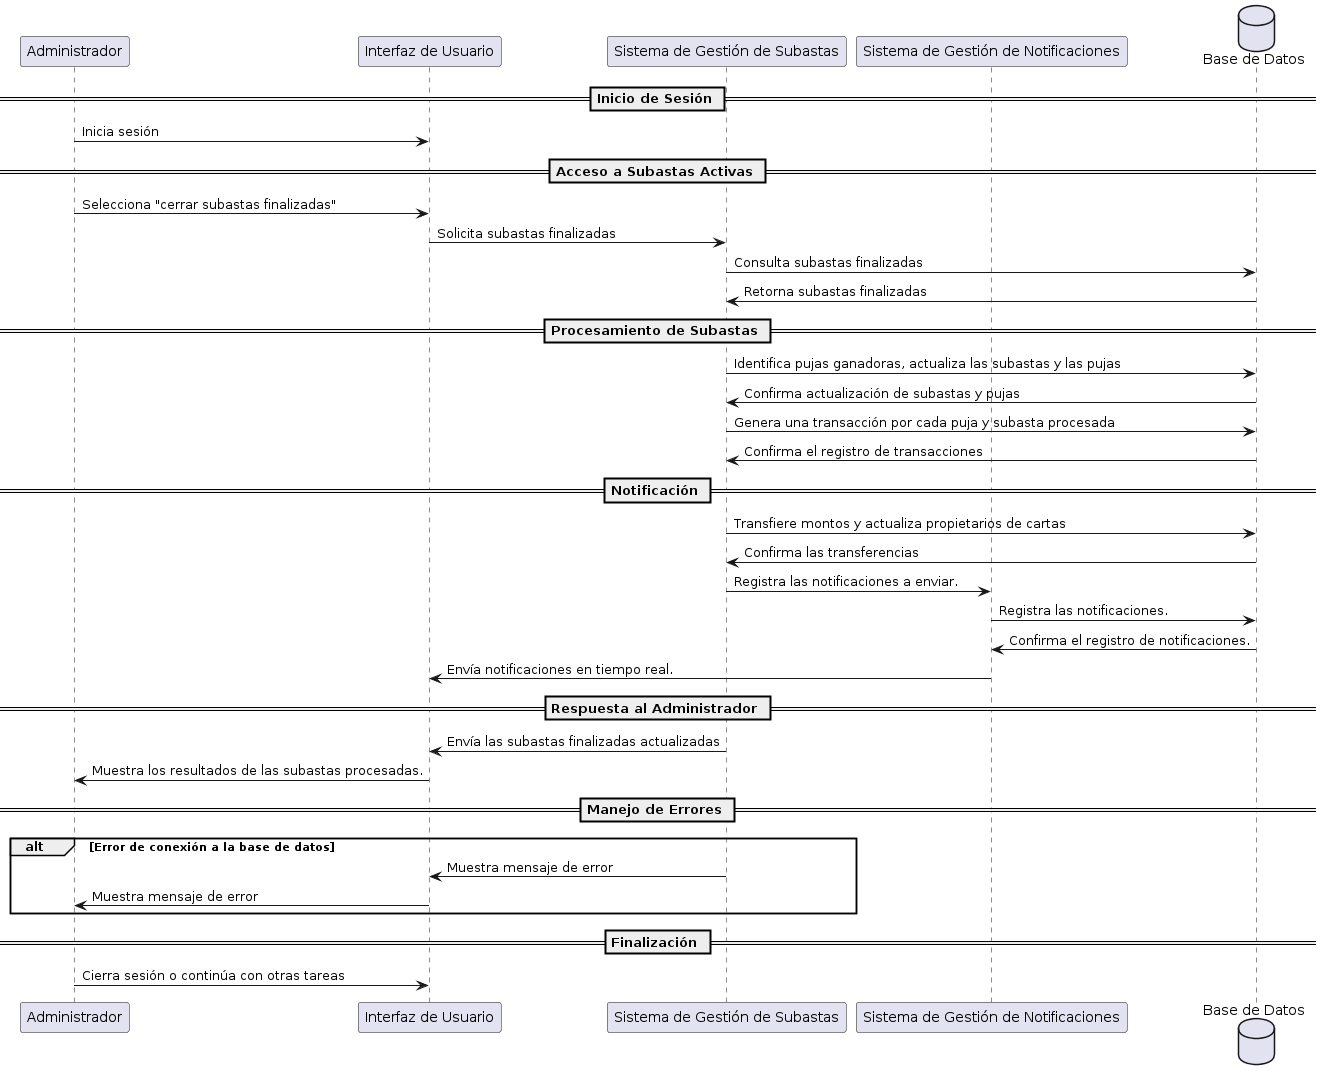
\includegraphics[width=1\textwidth]{figures/6-Analisis/6-Casos-uso/6_3_4_DSec-cerrar-subastas.png}
    \caption{Diagrama de secuencia. Cerrar subastas finalizadas}
    \label{fig:seq-cerrar-subastas}
\end{figure}